\begin{figure*}
\begin{center}

\begin{minipage}{0.15\linewidth}
\begin{subfigure}[b]{\linewidth}
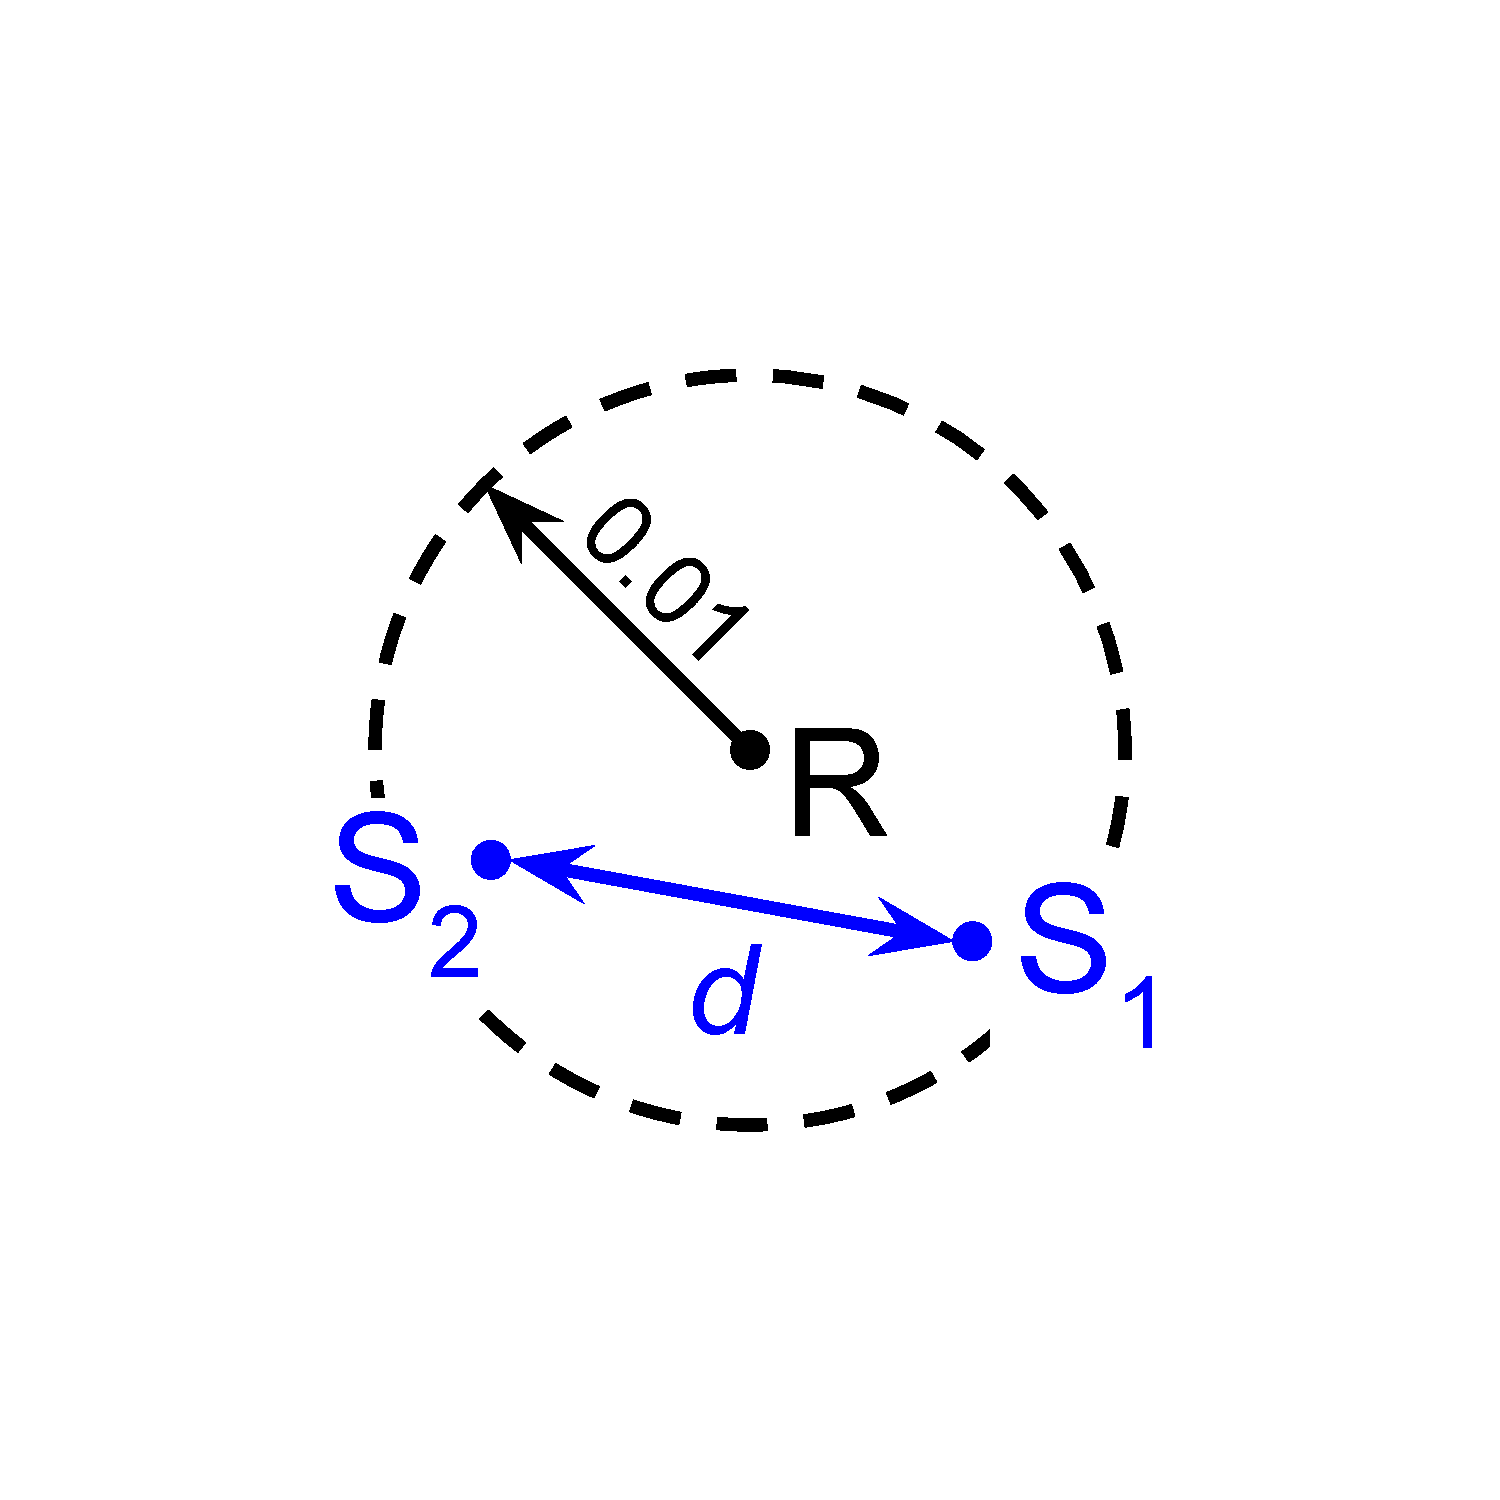
\includegraphics[width=\linewidth]{dimensionality-statistic}
\caption{
The sampling process used to calculate similarity constraint for each metric.
}
\end{subfigure}
\end{minipage}%
\begin{minipage}{0.35\textwidth}
\begin{subfigure}[b]{\linewidth}
\centering
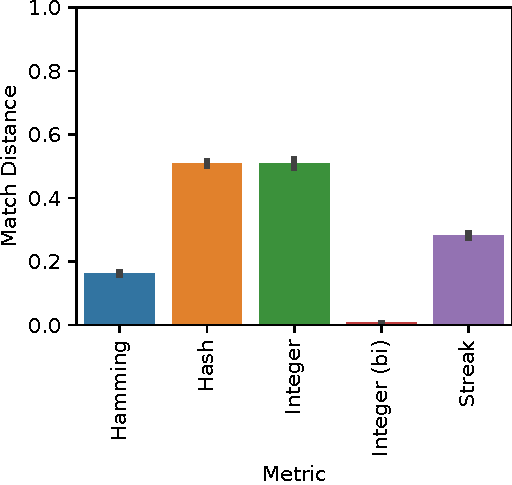
\includegraphics[width=\linewidth]{sphere/bitweight=0dot5+seed=1+title=dimensionality_barplot+_data_hathash_hash=c0f6c5cf854ff253+_script_fullcat_hash=03ce1e318a24a109+ext=}
\caption{
Mean statistic values for each metric.
Error bars represent 95\% confidence intervals.
}
\label{fig:sphere_distnplot}
\end{subfigure}
\end{minipage}%
\begin{minipage}{0.5\linewidth}
\begin{subfigure}[b]{\linewidth}
\centering
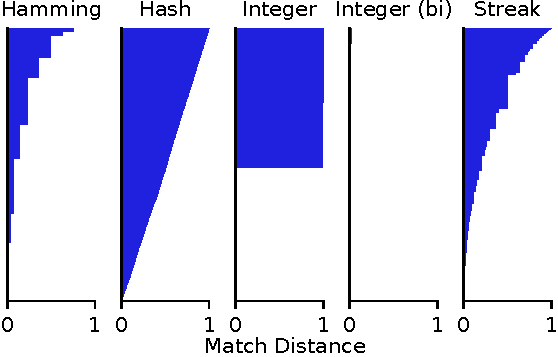
\includegraphics[width=\linewidth]{sphere/bitweight=0dot5+seed=1+title=dimensionality_distnplot+_data_hathash_hash=c0f6c5cf854ff253+_script_fullcat_hash=03ce1e318a24a109+ext=}
\caption{
Statistic distribution, where each horizontal bar sliver represents one independent observation.
}
\label{fig:sphere_barplot}
\end{subfigure}
\end{minipage}

\caption{
Dimensionality statistic measured as distances between two tags sampled from within 0.01 match distance of a third tag.
}
\label{fig:sphere}

\end{center}
\end{figure*}
